%%%%%%%%%%%%%%%%%%%%%%%%%%%%%%%%%%%%%%%%%%%%%%%%%%%%%%%%%%%%%%%%%%%%%%%%%%%%%%%%
%2345678901234567890123456789012345678901234567890123456789012345678901234567890
%        1         2         3         4         5         6         7         8

\documentclass[letterpaper, 10 pt, conference]{ieeeconf}  % Comment this line out if you need a4paper

%\documentclass[a4paper, 10pt, conference]{ieeeconf}      % Use this line for a4 paper

\IEEEoverridecommandlockouts                              % This command is only needed if 
                                                          % you want to use the \thanks command

\overrideIEEEmargins                                      % Needed to meet printer requirements.

% See the \addtolength command later in the file to balance the column lengths
% on the last page of the document

% The following packages can be found on http:\\www.ctan.org
%\usepackage{graphics} % for pdf, bitmapped graphics files
%\usepackage{epsfig} % for postscript graphics files
%\usepackage{mathptmx} % assumes new font selection scheme installed
%\usepackage{times} % assumes new font selection scheme installed
%\usepackage{amsmath} % assumes amsmath package installed
%\usepackage{amssymb}  % assumes amsmath package installed
\usepackage{graphicx}
\usepackage[export]{adjustbox}
\graphicspath{ {images/} }


\title{\LARGE \bf
Your Project Proposal Title
}


\author{Your Name$^{1}$ and Bernard D. Researcher$^{2}$% <-this % stops a space
\thanks{*This work was supported by the Robotics Master Program in National Chiao Tung University, Taiwan}% <-this % stops a space
\thanks{$^{1}$Your name is with National Chiao Tung University, Taiwan. You should put your name as first author
        {\tt\small youremail@papercept.net}}%
\thanks{$^{2}$You should add your teammates' names here,
        {\tt\small b.d.researcher@ieee.org}}%
}

\begin{document}

\maketitle
\thispagestyle{empty}
\pagestyle{empty}

\section{INTRODUCTION \& MOTIVATION}

There are five sections in this template, please follow the sections and feel free to add sub-sections. 

In this section, you need to give an introduction of your team's project started with a couple of sentences that introduce your topic to your readers. You do not have to give too much detailed information, but you explain why this project is important.

You should also have a literature review about relevant publications in BibTex format, for example, citing AprilTags~\cite{Olson09icra}. You should stand on giant's shoulder and know what have been done in the past. Recent papers in ICRA, IROS, RSS, CVPR, ICCV, ECCV, and etc. in the past 5 years, or a survey/review paper will be very helpful.

This IEEE template provides authors with most of the formatting specifications needed for preparing electronic versions of their papers. All standard paper components have been specified for three reasons: (1) ease of use when formatting individual papers, (2) automatic compliance to electronic requirements that facilitate the concurrent or later production of electronic products, and (3) conformity of style throughout a conference proceedings. Margins, column widths, line spacing, and type styles are built-in; examples of the type styles are provided throughout this document and are identified in italic type, within parentheses, following the example. Some components, such as multi-leveled equations, graphics, and tables are not prescribed, although the various table text styles are provided. The formatter will need to create these components, incorporating the applicable criteria that follow.

\begin{figure}[t]
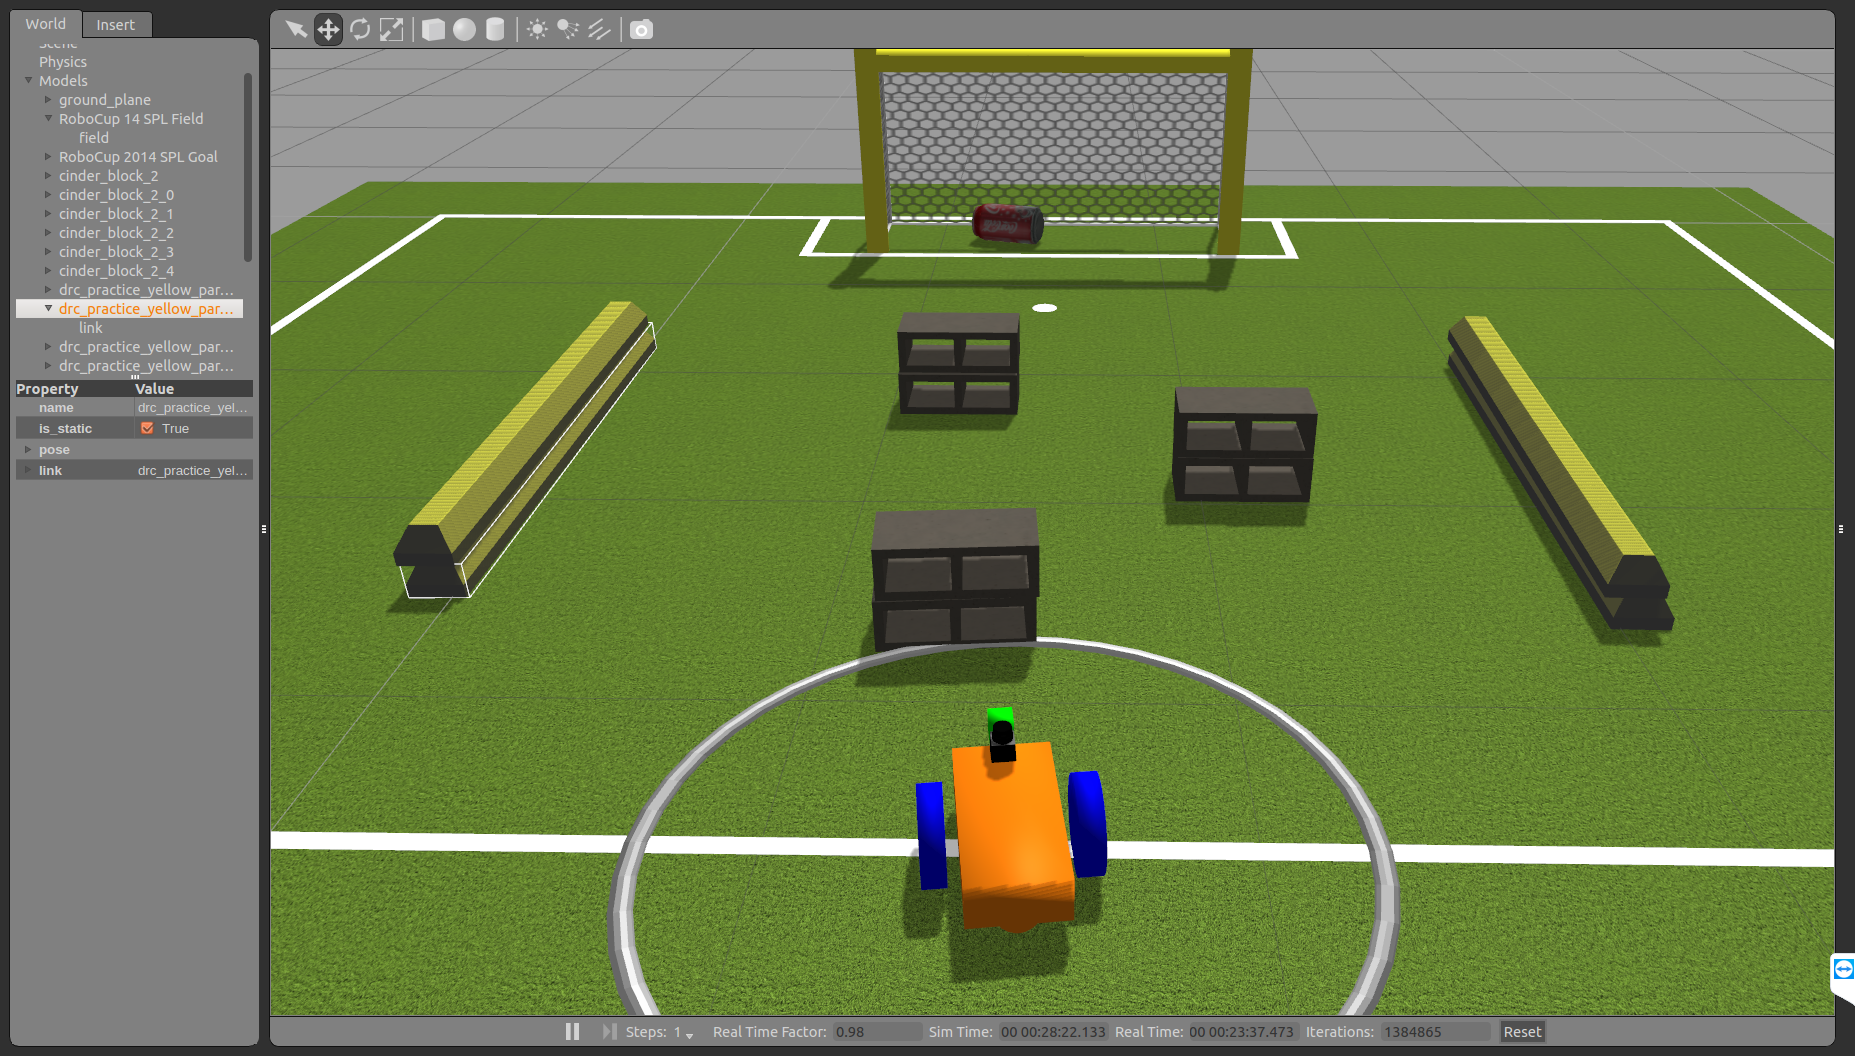
\includegraphics[width=0.95\columnwidth]{gazebo_view}
\centering
\caption{Teaser figure: this figure is the most important one in the paper. It gives your readers the first impression of this work. The teaser generally includes the overview of the proposed approach and the key contributions. It appears at the upper right of the first page.}
\end{figure}

\section{SYSTEM ARCHITECTURE \& EQUIPMENTS}

\subsection{SYSTEM ARCHITECTURE}

This section explains the approaches in both hardware or software systems. You should explain here the key components/modules and they are working together (typically in a flowchart). Wherever possible, the methods and tasks to be performed should be outlined in logical sequence and explained in detail. Do not assume the reviewer will fill in the gaps in your logic. 

\subsection{EQUIPMENTS} 

You should list the hardware which is necessary in your project. Your project will only become For example, UR5 collaborative robotics arm in Fig.~\ref{figure:ur5}, MIT2.12 mobile manipulators in Fig.~\ref{figure:mit212mm}, and Intel Realsense SR300~\ref{figure:sr300} ....

\begin{figure}[!b]
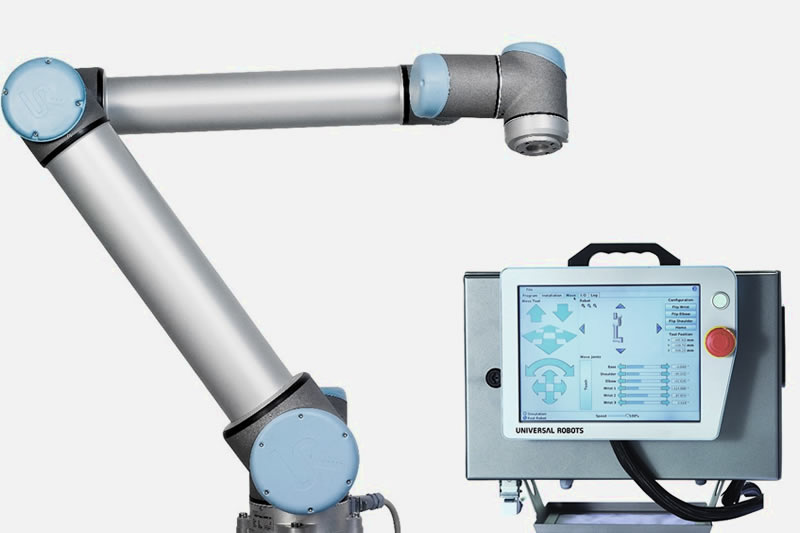
\includegraphics[width=0.7\columnwidth]{UR5}
\centering
\caption{UR5 robotic arm}
 \label{figure:ur5}
\end{figure}

\begin{figure}[h]
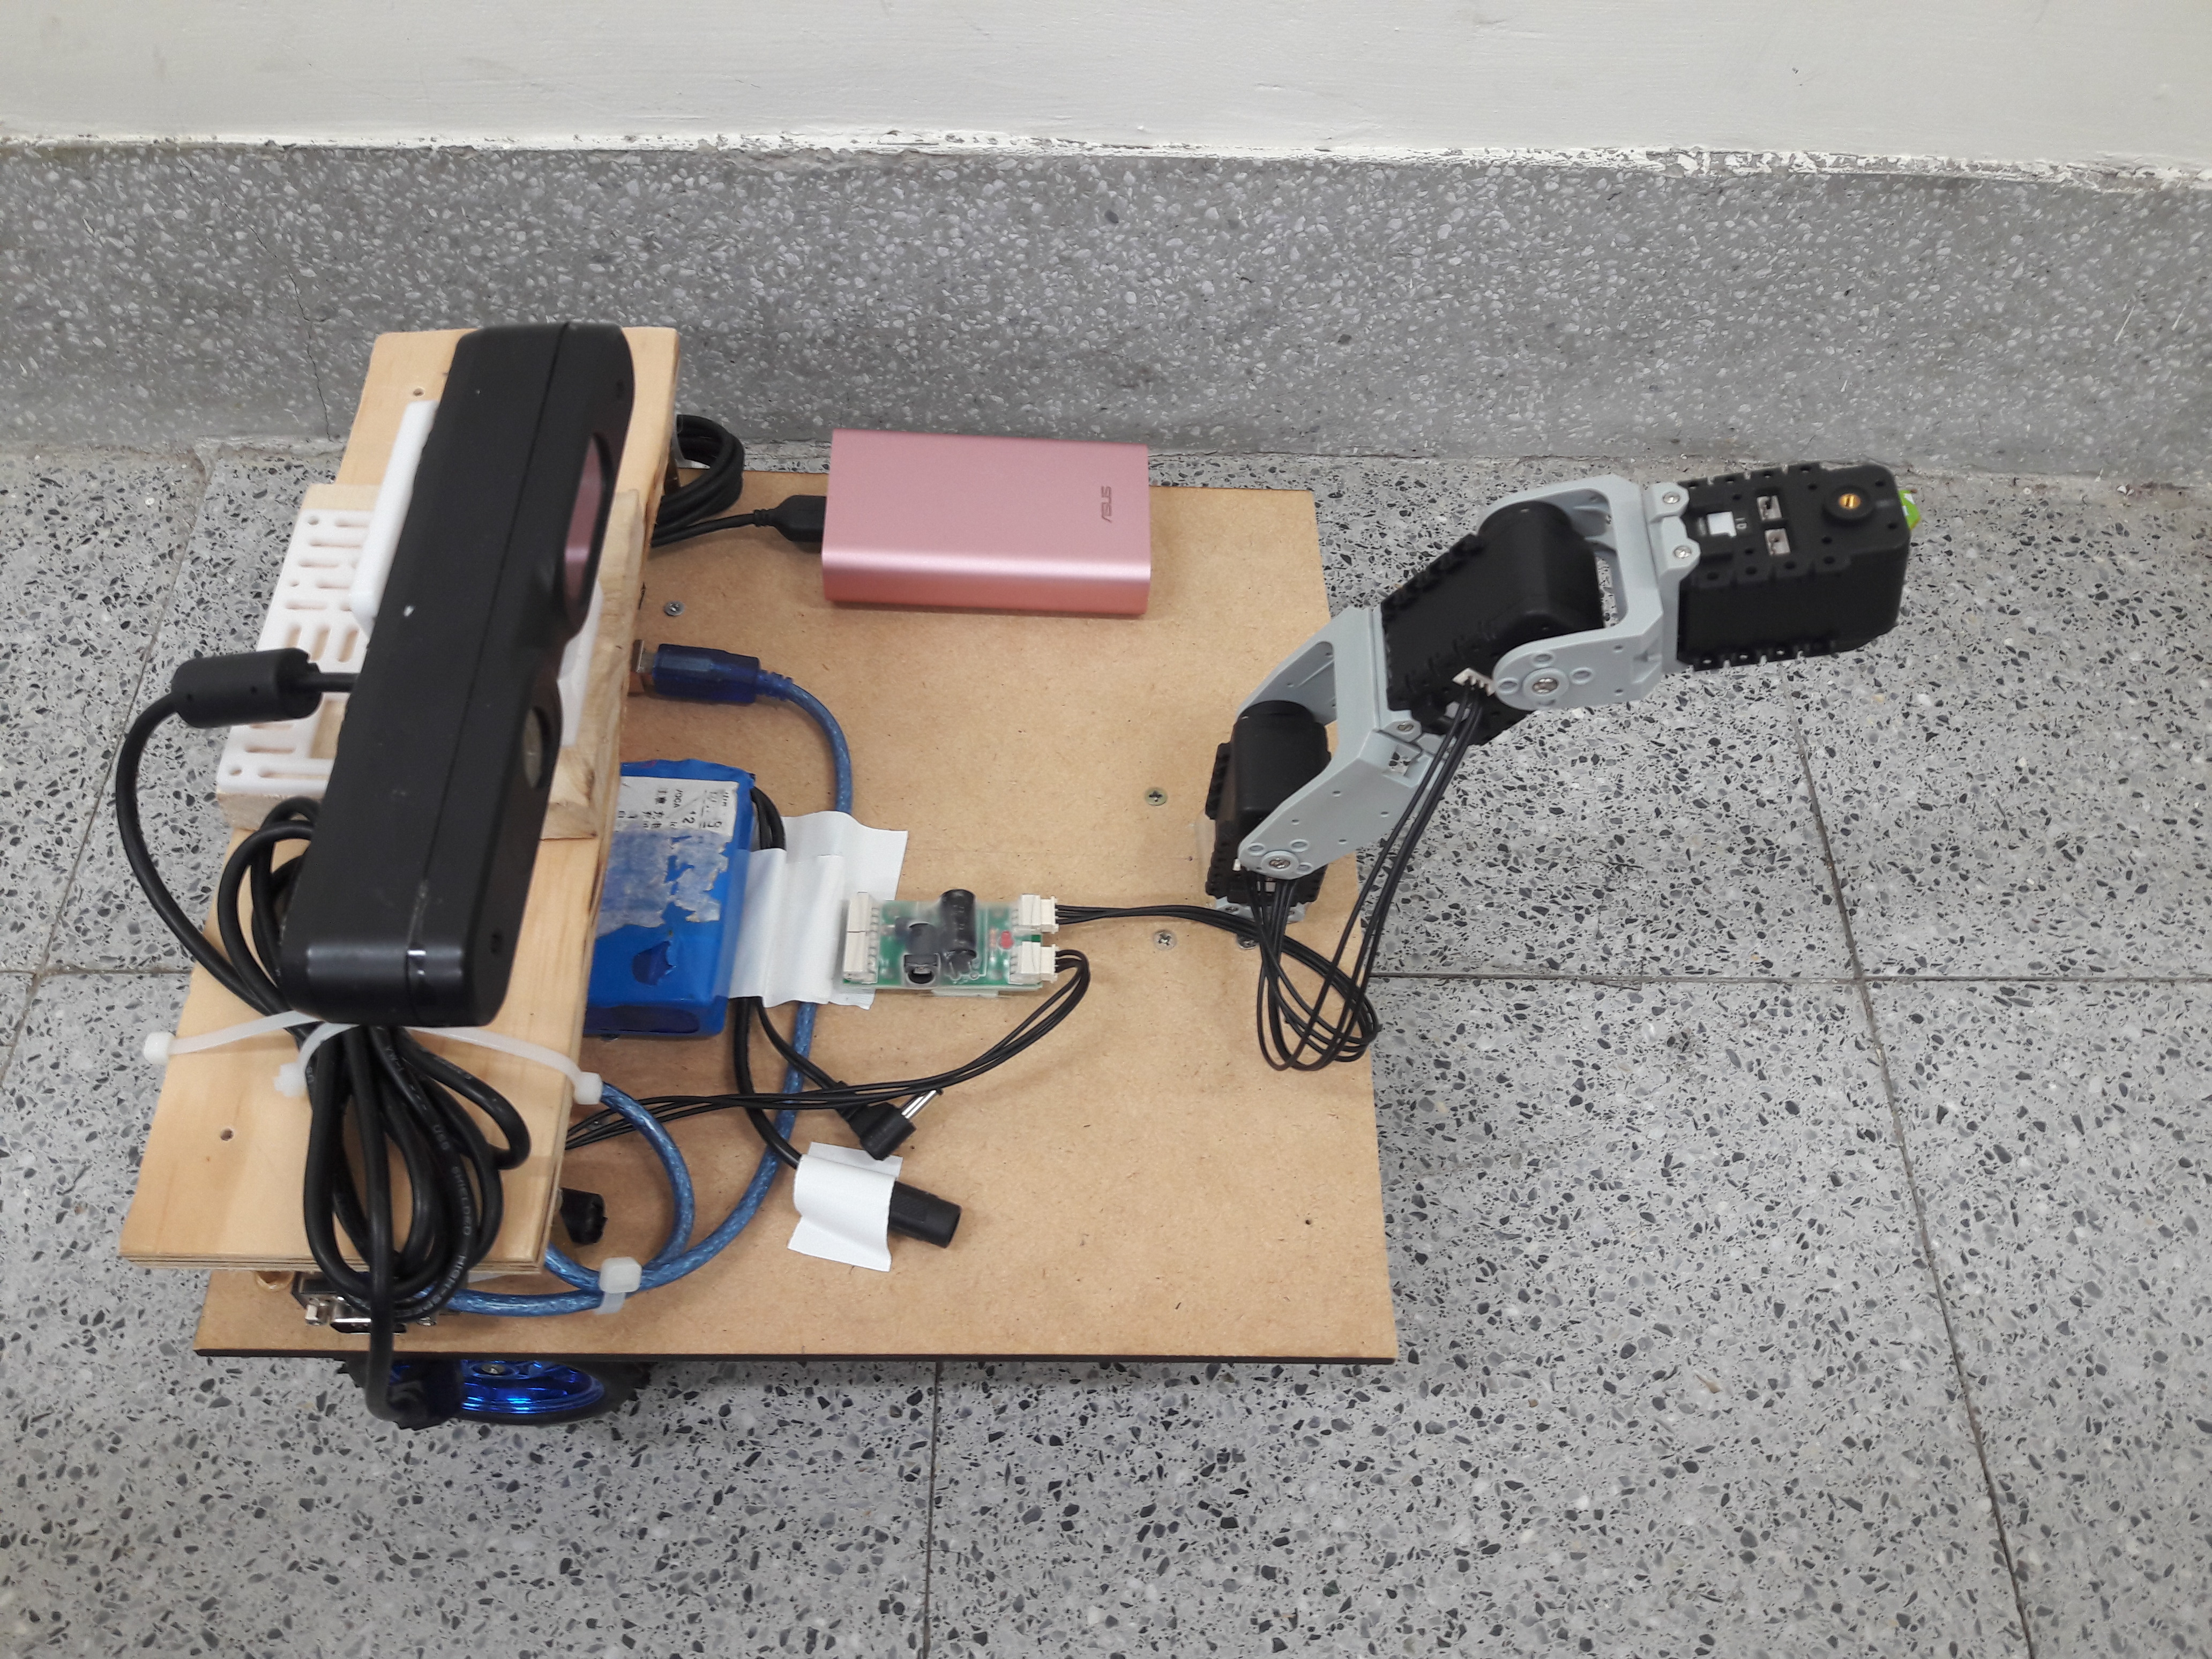
\includegraphics[width=0.7\columnwidth]{robot}
\centering
\caption{MIT2.12 Mobile Manipulator}
 \label{figure:mit212mm}
\end{figure}

\begin{figure}[h]
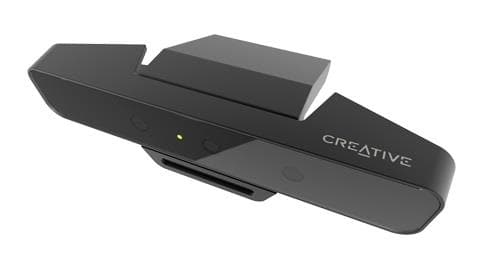
\includegraphics[width=0.7\columnwidth]{RealSense_Camera_SR300_SPL}
\centering
\caption{Intel Realsense SR300}
 \label{figure:sr300}
\end{figure}


\section{SPECIFIC AIMS}

Specific aims need to be concrete enough, so that it is clear what will be the expected outcomes of this work. You also need a reasonable scope that you could finish in this semester. For APC-focus group, the specific aims might be that you replicate a previous approach as baseline and do better in a component (such as the vision system). For the students who will use the 3 mobile manipulators, developing an additional module with a few tasks like our lab will be good. Each task could be a specific aim.

\section{APPROACH}

This section should include the methods that you will need in order to reach the specific aims. You could include how you will implement your software/hardware, the design of the algorithms. Some preliminary results will be helpful as well. 

You may also state what experiments you will carry out to convince the readers that you reach the specific aims.

\section{SCHEDULE AND TEAM COLLABORATION}

In this section you should write a estimated timeline of your project. This schedule will be very crucial to keep up progress for your project. If you are in a team, you're encouraged to add other team members' on the timeline. It will better show the coordination of your team.
   

\bibliographystyle{IEEEtran}
\bibliography{arg-egbib}

\end{document}
